\documentclass[a4paper,11pt,oneside]{article}

\usepackage[utf8]{inputenc}
\usepackage[T1]{fontenc}
\usepackage[ngerman]{babel}
\usepackage{amssymb}
\usepackage{amsmath}
\usepackage{graphicx}
\usepackage{float}
\usepackage{hyperref}
\usepackage[dvipsnames]{xcolor}
\usepackage{listings}
\usepackage[top=2cm, bottom=2.5cm, right=2.5cm, left=2.5cm]{geometry}

\renewcommand{\familydefault}{\sfdefault}
\parindent0pt
\parskip6pt
\hypersetup{colorlinks=true,urlcolor=blue,linkcolor=blue}
\lstset{basicstyle=\ttfamily\small, mathescape, literate={Ö}{{\"O}}1 {Ä}{{\"A}}1 {Ü}{{\"U}}1 {ß}{{\ss}}1 {ü}{{\"u}}1 {ä}{{\"a}}1 {ö}{{\"o}}1}

\begin{document}

\title{Wahrscheinlichkeit an der kürzeren Warteschlange länger warten zu müssen}
\author{Alexander Herzog\\\href{mailto:alexander.herzog@tu-clausthal.de}{\small\texttt{alexander.herzog@tu-clausthal.de}}}
\date{}

\maketitle

Stehen z.\,B.\ im Supermarkt mehrere Kassen zur Auswahl, so neigt man dazu, sich bei der Kasse mit der kürzesten Warteschlange anzustellen, um die eigene Wartezeit zu minimieren.

Aus Erfahrung weiß man jedoch, dass diese Strategie nicht immer zielführend ist. Da die Bediendauern der einzelnen Kunden zufälligen Schwankungen unterliegen (der eine hat mehr im Einkaufskorb, der andere weniger; Bezahlvorgänge dauern unterschiedlich lange), kann es vorkommen, dass an der längeren Warteschlange zufällig viele schnell abzuarbeitende Aufträge aufeinander folgen, während an der kürzeren Schlange zeitlich aufwändigere Aufträge überwiegen. In diesem Fall muss man an der kürzeren Schlange möglicherweise länger warten als an der längeren Schlange.

Mathematisch lässt sich zeigen, dass diese Situation umso häufiger eintritt
\begin{itemize}
\item je unregelmäßiger die Arbeitsaufträge der einzelnen Kunden sind,
\item je mehr Kunden in den Warteschlangen stehen und
\item je kleiner der Unterschied in der Länge der Warteschlangen ist.
\end{itemize}

Sind umgekehrt alle Arbeitsaufträge gleich aufwändig, so wird man an der Kasse mit der kürzeren Warteschlange gesichert auch schneller abgefertigt werden.



\section{Mathematische Formulierung des Problems}

Um analytisch zu berechnen, wie groß die Wahrscheinlichkeit ist, dass man an der kürzeren Warteschlange länger warten muss als an der längeren, wählen wir die folgenden Bezeichnungen:

\begin{itemize}
\item
Wir treffen in einem Supermarkt am Kassenbereich ein. Zwei Kassen sind geöffnet (und an jeder geöffneten Kasse arbeitet ein Bediener, es gilt also zwei mal $c=1$).
\item
Die Bedienrate betrage an beiden Kassen $\mu>0$. Die Bedienzeiten seien exponentiell verteilt. Es gibt also keine strukturellen Unterschiede zwischen den Kassen in Bezug auf die Bediendauern. (Von außen ersichtliche strukturelle Unterschiede wären z.\,B.\ wenn eine Kasse eine ,,maximal 3 Teile''-Kasse ist oder eine Kasse explizit für nur Barzahlungen oder nur für Kartenzahlungen eingerichtet ist.)
\item
An der ersten Kasse befinden sich zum Zeitpunkt unseres Eintreffens $a\in\mathbb{N}$ Personen; an der zweiten Kasse $b\in\mathbb{N}$. Die Anzahl umfasst jeweils die wartenden Kunden und den Kunden in Bedienung.
\item
Es sei $a>b$, d.\,h.\ an der ersten Kasse befinden sich mehr Personen als an der zweiten. Da die Bediendauern an den beiden Kassen keinen systematischen Unterschieden unterliegen, ist es naheliegend, die zweite Kasse zu favorisieren.
\end{itemize}

Gesucht ist die Wahrscheinlichkeit dafür, an der zweiten Kassen länger warten zu müssen, als dies an der ersten Kasse der Fall gewesen wäre, d.\,h.\ mathematisch formuliert:

$$
P(W_{(b)}>W_{(a)})
$$
(trotz $b<a$).



\section{Exponentialverteilung}

Im Folgenden wird es darum gehen, die Verteilung für die eigene Bediendauer in Abhängigkeit von der Wahl der Warteschlange zu bestimmen. Die eigene Bediendauer setzt sich aus der Restbediendauer des aktuell in Bearbeitung befindlichen Kunden und der Summe der Bediendauern aller anderen Kunden vor uns in der Warteschlange zusammen.

Die Bediendauern der wartenden Kunden (deren Bedienungen noch nicht begonnen haben) unterliegen gemäß der obigen Annahme der Exponentialverteilung. Um die Faltung der einzelnen Zeitdauern berechnen zu können, muss also noch die Verteilung der Restbediendauer des aktuell in Bearbeitung befindlichen Kunden bestimmt werden.

Für die Verteilungsfunktion $F(t)$ der Exponentialverteilung gilt:
$$
P(X\le t)=F(t)=1-e^{-\mu t} \quad\text{für}\quad t\geq0.
$$
Für die Restbediendauer einen Kunden, der bereits $t_0\ge0$ Zeiteinheiten bedient wurde, gilt gemäß der Definition der bedingten Wahrscheinlichkeit:
\begin{eqnarray*}
P(X\le t+t_0|X\ge t_0)
&=&\frac{P(\{X\le t+t_0\}\cap \{X\ge t_0\})}{P(X\ge t_0)}
 = \frac{P(t_0\le X\le t+t_0)}{P(X\ge t_0)}\\
&=&\frac{F(t+t_0)-F(t_0)}{1-F(t_0)}\\
&=&\frac{(1-e^{-\mu(t+t_0)})-(1-e^{-\mu t_0})}{1-(1-e^{-\mu t_0})}
 = \frac{-e^{-\mu t}\cdot e^{-\mu t_0}+e^{-\mu t_0}}{e^{-\mu t_0}}\\
&=&1-e^{-\mu t}
 = F(t)=P(X\le t).
\end{eqnarray*}
Das bedeutet, die Wahrscheinlichkeit, dass die Restbediendauer eines Kunden, der bereits $t_0$ Zeiteinheiten bedient wurde, kleiner oder gleich $t$ ist, entspricht der Wahrscheinlichkeit, dass die Bediendauer eines neu ankommenden Kunden kleiner oder gleich $t$ ist. Mit anderen Worten: Die Restbediendauer eines Kunden, der bereits $t_0$ Zeiteinheiten bedient wurde, ist ebenfalls exponentiell verteilt mit dem gleichen Verteilungsparameter $\mu$. Wie lange der Kunde bereits bedient wurde, spielt also (wenn die Exponentialverteilung für die Bediendauern angenommen wird) für seine Restbediendauer keine Rolle. Diese Eigenschaft der Exponentialverteilung wird auch als \emph{Gedächtnislosigkeit} bezeichnet.



\section{Faltung der Exponentialverteilung}

Wir wissen nun also, dass die eigene Wartezeit an einer Kasse, an der sich $n$ Kunden vor uns befinden ($n-1$ wartend und einer in Bedienung), sich aus der Summe von $n$ exponentiell verteilten Zufallsvariablen zusammensetzt. Gesucht ist folglich die Verteilung der Summe von $n$ unabhängigen, exponentiell verteilten Zufallsvariablen $X_1,\ldots,X_n$.

Die Dichte der Verteilung, die sich als Summe von zwei Verteilungen (mit Dichten $f$ und $g$) ergibt, wird mit $f*g$ bezeichnet und wie folgt berechnet:
$$
(f*g)(x)=\int_{-\infty}^{\infty} f(x-y)g(y)\,dy.
$$
Dieser Vorgang wird die \emph{Faltung} der Dichten genannt. Die Dichte der Verteilung der eigenen Wartezeit ist also die $n$-fache Faltung der Dichte der Exponentialverteilung. Die $n$-fache Faltung einer Dichte $f$ mit sich selbst wird mit $f^{*n}$ bezeichnet.

Per Induktion lässt sich nachrechnen, dass die $n$-fache Faltung der Dichte der Exponentialverteilung mit Parameter $\mu$ die Dichte der \emph{Erlang-Verteilung} mit den Parametern $n$ und $\mu$ ergibt. Für Dichte und Verteilungsfunktion der Erlang-Verteilung gelten:
\begin{eqnarray*}
f_{\mu,n}(t)&=&\frac{t^{n-1}e^{-\frac{t}{\mu}}}{\mu^n(n-1)!},\\
F_{\mu,n}(t)&=&1-e^{-\frac{t}{\mu}}\cdot\sum_{k=0}^{n-1}\frac{1}{k!}\left(\frac{t}{\mu}\right)^k \quad\text{für}\quad t\geq0.
\end{eqnarray*}

Die Wahrscheinlichkeit, in einem Bediensystem mit $c=1$ Bediener und $n\in\mathbb{N}$ Kunden \emph{länger} als $t\ge0$ Sekunden warten zu müssen, ist damit:

$$
P(W_{(n)}>t)=
1-P(W_{(n)}\le t)=
1-F_{\mu,n}(t)=
e^{-\mu t}\cdot\sum_{k=0}^{n-1}\frac{(\mu t)^k}{k!}.
$$



\section{Bedingte Verteilung}

Bei der gesuchten Größe $P(W_{(b)}>W_{(a)})$ handelt es sich um eine bedingte Verteilung: Normalerweise wird gefragt, wie groß die Wahrscheinlichkeit, dass der Wert einer Zufallsvariablen $X$ kleiner oder größer als eine feste Zahl $t$ ist. Hier werden jedoch zwei Zufallsvariablen $W_{(a)}$ und $W_{(b)}$ in Beziehung gesetzt. Diese Wahrscheinlichkeit lässt sich über die \emph{bedingte Verteilung} berechnen:

\begin{eqnarray*}
P(W_{(b)}>W_{(a)})&=&
\int_{\mathbb{R}^+}P(W_{(b)}>W_{(a)}|W_{(a)}=t)\cdot f_{W_{(a)}}(t)~dt\\
~&=&
\int_{\mathbb{R}^+}P(W_{(b)}>t)\cdot f_{W_{(a)}}(t)~dt\\
~&=&
\int_{\mathbb{R}^+}
\left(e^{-\mu t}\cdot\sum_{k=0}^{b-1}\frac{(\mu t)^k}{k!}\right)\cdot\left(\frac{\mu^at^{a-1}e^{-\mu t}}{(a-1)!}\right)~dt\\
~&=&
\frac{\mu^{a-1}}{(a-1)!}\cdot\int_{\mathbb{R}^+}\sum_{k=0}^{b-1}\frac{(\mu t)^k}{k!}\cdot t^{a-1}\cdot\mu\cdot e^{-2\mu t}~dt\\
~&=&
\frac{1}{2}\cdot\frac{\mu^{a-1}}{(a-1)!}\cdot\int_{\mathbb{R}^+}\sum_{k=0}^{b-1}\frac{(\mu t)^k}{k!}\cdot t^{a-1}\cdot2\mu\cdot e^{-2\mu t}~dt\\
~&=&
\frac{1}{2}\cdot\frac{\mu^{a-1}}{(a-1)!}\cdot\sum_{k=0}^{b-1} \frac{\mu^k}{k!}\int_{\mathbb{R}^+}t^{a+k-1}\cdot2\mu\cdot e^{-2\mu t}~dt.
\end{eqnarray*}



\section{Momente der Exponentialverteilung}

Wir wollen uns nun den Ausdruck
$$
\int_{\mathbb{R}^+}t^{a+k-1}\cdot2\mu\cdot e^{-2\mu t}~dt
$$
näher ansehen:

\begin{itemize}
\item Es waren $a>b$ und $a,b\in\mathbb{N}$, d.\,h.\ $a\ge2$. Damit ist $n:=a+k-1\in\mathbb{N}$ für alle $k\in\mathbb{N}_0$.
\item Weiter sei zur Abkürzung $\tilde\mu:=2\mu$.
\end{itemize}

Damit können wir den obigen Ausdruck schreiben als:
$$
\int_{\mathbb{R}^+}t^{n}\cdot\tilde\mu\cdot e^{-\tilde\mu t}~dt.
$$
Das ist aber gerade das $n$-te Moment der Exponentialverteilung mit Parameter $\tilde\mu$:
$$
\mathbf{E}[X_{\tilde\mu}^n]=
\int_{\mathbb{R}^+}t^{n}\cdot\tilde\mu\cdot e^{-\tilde\mu t}~dt=
\int_{\mathbb{R}^+}t^{n} f_{\tilde\mu}(t)~dt
$$
(mit $f_{\tilde\mu}(t):=\tilde\mu\cdot e^{-\tilde\mu t}$). Per Induktion lässt sich zeigen, dass für die Momente der Exponentialverteilung mit Parameter $\tilde\mu$ gilt:
$$
\mathbf{E}[X_{\tilde\mu}^n]=\frac{n!}{\tilde\mu^n}.
$$
Hier also:
$$
\int_{\mathbb{R}^+}t^{a+k-1}\cdot2\mu\cdot e^{-2\mu t}~dt=
\mathbf{E}[X_{2\mu}^{a+k-1}]=\frac{(a+k-1)!}{(2\mu)^{a+k-1}}.
$$



\section{Endgültige Berechnung der gesuchten Wahrscheinlichkeit}

Mit den obigen Überlegungen lässt sich die gesuchte Wahrscheinlichkeit $P(W_{(b)}>W_{(a)})$ jetzt berechnen:

\begin{eqnarray*}
P(W_{(b)}>W_{(a)})&=&
\frac{1}{2}\cdot\frac{\mu^{a-1}}{(a-1)!}\cdot\sum_{k=0}^{b-1} \frac{\mu^k}{k!}\int_{\mathbb{R}^+}t^{a+k-1}\cdot2\mu\cdot e^{-2\mu t}~dt\\
~&=& \frac{1}{2}\cdot\frac{\mu^{a-1}}{(a-1)!}\cdot\sum_{k=0}^{b-1} \frac{\mu^k}{k!} \frac{(a+k-1)!}{(2\mu)^{a+k-1}}\\
~&=& \frac{1}{2}\cdot\frac{1}{(a-1)!}\cdot\sum_{k=0}^{b-1}\frac{1}{k!}\cdot\frac{(a+k-1)!}{2^{a+k-1}}\\
~&=& \left(\frac{1}{2}\right)^a\cdot\sum_{k=0}^{b-1}\frac{(a+k-1)!}{k!\cdot(a-1)!}\cdot\left(\frac{1}{2}\right)^k.
\end{eqnarray*}

Mit der Definition des Binomialkoeffizienten
$$
\binom{n}{k}:=\frac{n!}{k!\cdot(n-k)!}
$$
folgt das Endergebnis:

\begin{eqnarray}
\nonumber
P(W_{(b)}>W_{(a)})&=&
\left(\frac{1}{2}\right)^a\cdot\sum_{k=0}^{b-1}\frac{(a+k-1)!}{k!\cdot(a-1)!}\cdot\left(\frac{1}{2}\right)^k\\
~&=&
\left(\frac{1}{2}\right)^a\cdot\sum_{k=0}^{b-1}\binom{a+k-1}{k}\cdot\left(\frac{1}{2}\right)^k.
\label{eq:PWbBiggerThanWa}
\end{eqnarray}




\section{Implementierung in Python}

Die Ergebnisformel \eqref{eq:PWbBiggerThanWa} lässt sich einfach in Python implementieren. Dabei wird die Funktion \texttt{binom} aus dem Modul \texttt{scipy.special} verwendet, um den Binomialkoeffizienten zu berechnen. Die Funktion \texttt{PWbBiggerThanWa(a, b)} berechnet die Wahrscheinlichkeit, an einer Kasse, an der sich $b$ Kunden befinden, länger warten zu müssen als an einer Kasse, an der sich $a$ Kunden befinden (mit $a>b$ und Annahme der Exponentialverteilung für die Bediendauern):

\vskip0.5em
\begin{lstlisting}[inputencoding={utf8},frame=single]
from scipy.special import binom

def PWbBiggerThanWa(a, b):
    assert a > b, "a muss größer als b sein"
    return 0.5**a*sum([binom(a+k-1, k)*0.5**k for k in range(b)])
\end{lstlisting}
\vskip0.5em

Variiert man $b$ (die Länge der kürzeren Warteschlange) im Bereich von 1 bis 25 und wählt $a:=b+1$, $a:=b+2$ und $a:=b+3$, so ergeben sich die in Abbildung \ref{fig:PWbBiggerThanWa} dargestellten Graphen.

\begin{figure}[H]
\centering
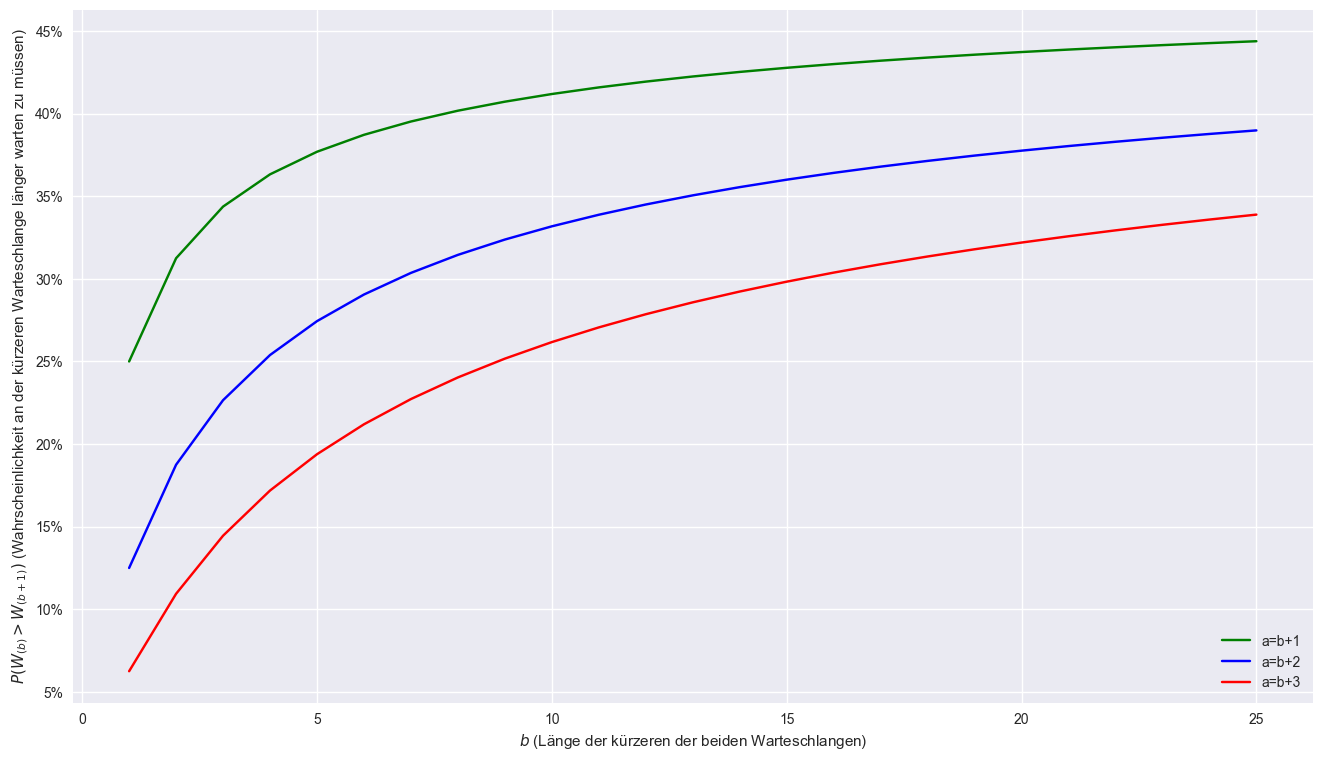
\includegraphics[width=0.99\textwidth]{KuerzereWarteschlange.png}
\caption{Wahrscheinlichkeit, an der kürzeren Warteschlange länger warten zu müssen}
\label{fig:PWbBiggerThanWa}
\end{figure}

Es ist deutlich zu erkennen, dass die Wahrscheinlichkeit, an der kürzeren Warteschlange länger warten zu müssen (hohe $y$-Werte), umso größer wird, je kleiner der Unterschied in der Länge der Warteschlangen ist (grüner Graph) und auch je länger die beiden betrachteten Warteschlangen insgesamt sind (große $x$-Werte).

Interaktiv ausprobieren lässt sich dieses Verhalten auf der folgenden Webseite:\\
\href{https://a-herzog.github.io/QueueCalc/?function=ShortestQueueValues}{a-herzog.github.io/QueueCalc/?function=ShortestQueueValues}

\end{document}
